\section{Durchsatz, Energie und Qualität der gemessenen Konfigurationen}
\label{app:model_tradeoffs}

Die folgenden Abbildungen erweitern die ausgewählten Vergleiche aus Kapitel~\ref{sec:evaluation} auf den gesamten Messraum für jedes Modell. Sie zeigen die 450 Konfigurationen mit Durchsatz- und Energiebeobachtungen über die drei Aufbauten hinweg. Darunter befinden sich 43 Konfigurationen, die außerhalb der primären 5\%-Grenze für Qualitätsverlust liegen. Die Konfiguration Generic YOLOv7/H8 b009 weist keinen Energiewert auf und wird daher in diesen Diagrammen nicht berücksichtigt. Durchsatz, Energieverbrauch und numerische Qualität können somit vor der Filterung überprüft werden~\cite{edgeAIResults2026}.

Jeder Punkt steht für eine Ausführungskonfiguration mit dem aufgezeichneten prozessbezogenen Median-Durchsatz und der mittleren kalibrierten Energie (einschließlich Host) pro fertiggestelltem Bild. Die Form der Markierung unterscheidet die beiden geteilten Implementierungen und die beiden Full-Alternativen. Die Farbe zeigt die numerische Top-1-Genauigkeit oder den aufgezeichneten AP$_{50:95}$ an. Die Detektormetrik ist COCO AP$_{50:95}$. Die drei vertikal angeordneten Felder für jedes Modell verwenden eine gemeinsame Farbskala, ihre Achsen sind jedoch separat skaliert. Die Farben lassen sich nicht über verschiedene Modelle oder Aufgaben hinweg vergleichen.

Schwarze Konturen markieren die Durchsatz-Energie-Grenze für jedes Modell und jeden Beschleuniger. Eine Konfiguration liegt auf dieser Grenze, wenn keine andere gemessene Alternative eine Metrik verbessert, ohne die andere zu verschlechtern. Bei Verwendung ungerundeter Werte und unter Berücksichtigung von Gleichständen ergeben sich 34 Konfigurationen in 21 Kombinationen. Die Bestimmung dieser Grenze erfolgt ohne Qualitätsfilterung. Die Farbe zeigt die Qualität separat an, sodass bei einer Einsatzentscheidung auch das erforderliche Qualitätsniveau überprüft werden muss. Die Abbildungen beschreiben gemessene Alternativen unter Berücksichtigung ihrer tatsächlichen Laufzeitumgebungen und Ablaufsteuerungen. Sie legen keine Dominanz bei gleicher Qualität oder erreichbaren Zwischenkonfigurationen fest.

Das Auswertungswerkzeug generiert diese Ansichten aus derselben numerischen Tabelle wie der Einsatzvergleich. Dazu gehört YOLO11l/DeepX b511 mit seiner gemessenen Generic-Energie. Die Bezeichnungen F und E kennzeichnen die schnellste bzw. die energieeffizienteste Ausführungskonfiguration für ein Ausführungsmodul. N steht für Native und G für Generic. Geringe Abweichungen sollten im Zusammenhang mit den beobachteten Wiederholungen und den in den Hauptkapiteln erörterten Messgrenzen betrachtet werden.

\clearpage
\begin{figure}[p]
\centering
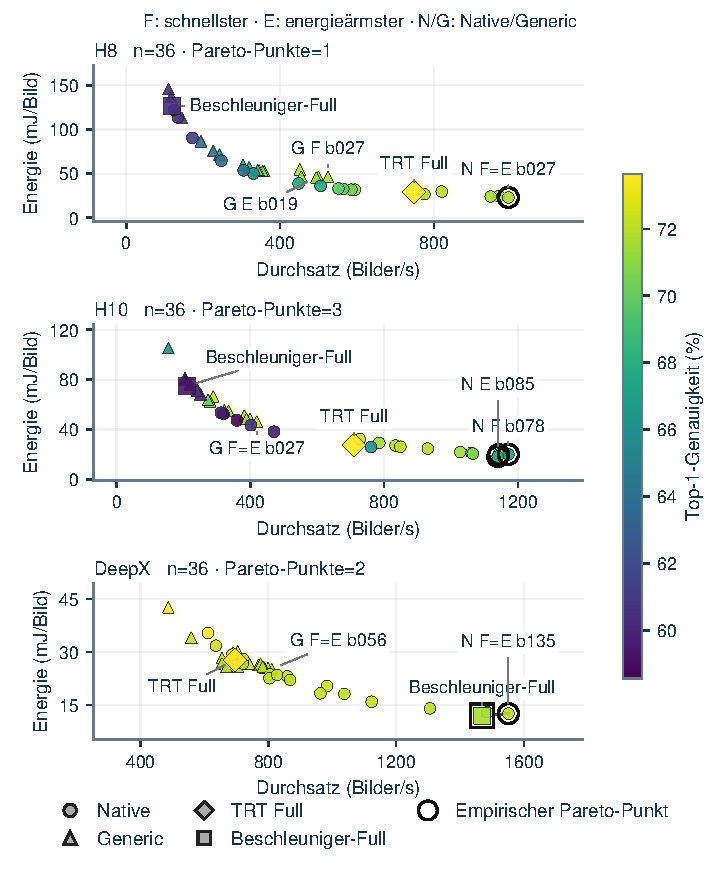
\includegraphics[width=4.8in]{9_resources/10_anhang/04_tradeoff_mobilenet_v3_large.pdf}
\caption[MobileNetV3-Konfigurationsraum]{MobileNetV3 Large: 108 gemessene Ausführungskonfigurationen. Die drei lokalen Zwei-Ziel-Grenzen enthalten einen, drei bzw. zwei Punkte. Die schnellste Split-Variante läuft auf DeepX. Ihr bescheidener Durchsatzvorteil gegenüber der schnellsten Full-Konfiguration über alle untersuchten Systeme bringt keine Energieeinsparung mit sich. Schwarze Umrisse markieren die ungefilterte Grenze.}
\label{fig:gallery:mobilenet}
\end{figure}
\clearpage
\begin{figure}[p]
\centering
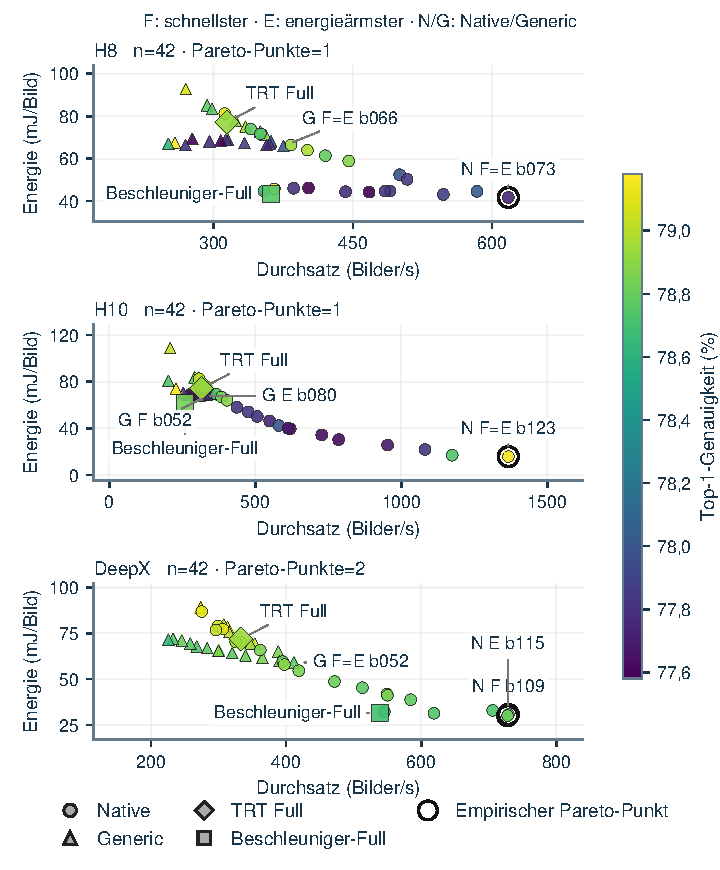
\includegraphics[width=4.8in]{9_resources/10_anhang/04_tradeoff_regnet_x_1_6gf.pdf}
\caption[RegNet-X-Konfigurationsraum]{RegNet-X 1.6GF: 126 gemessene Ausführungskonfigurationen. H8 und H10 weisen jeweils einen Grenzpunkt mit zwei Zielgrößen auf, DeepX weist zwei solche Punkte auf. Die H10-Split-Konfiguration liefert unter den Hauptoptionen die stärkste kombinierte Verbesserung bei Durchsatz und Energieverbrauch. Die Diagramme enthalten alle erfassten numerischen Qualitätsstufen.}
\label{fig:gallery:regnet}
\end{figure}
\clearpage
\begin{figure}[p]
\centering
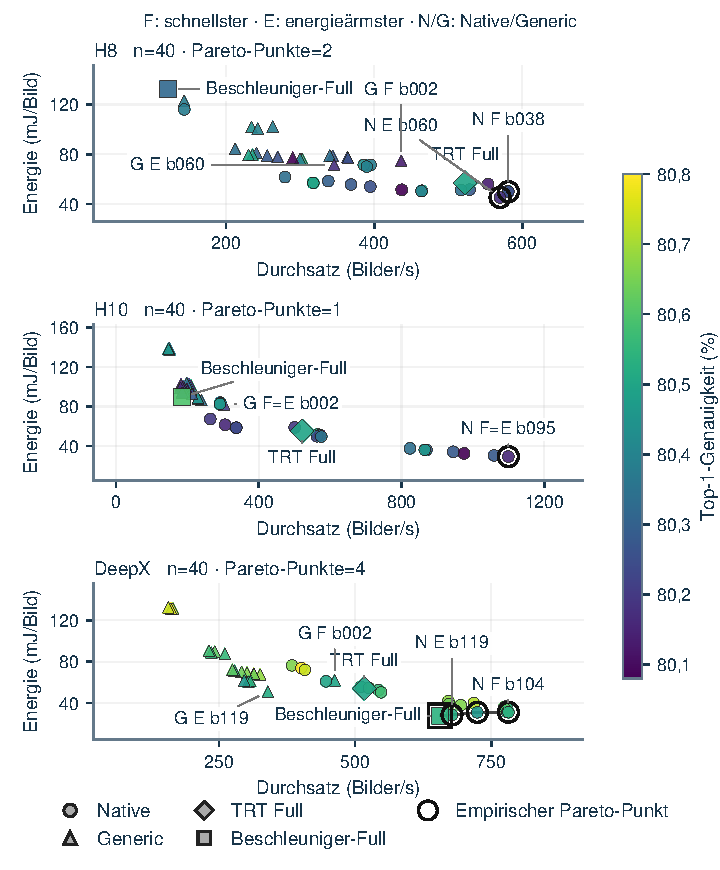
\includegraphics[width=4.8in]{9_resources/10_anhang/04_tradeoff_resnet50.pdf}
\caption[ResNet-50-Konfigurationsraum]{ResNet-50: 120 gemessene Ausführungskonfigurationen. H8 und DeepX bieten mehrere lokale Auswahlmöglichkeiten zwischen Durchsatz und Energieverbrauch. Die über alle untersuchten Systeme schnellste Split-Variante auf H10 übertrifft die schnellste Full-Konfiguration über alle untersuchten Systeme beim Durchsatz, verbraucht jedoch mehr Energie.}
\label{fig:gallery:resnet}
\end{figure}
\clearpage
\begin{figure}[p]
\centering
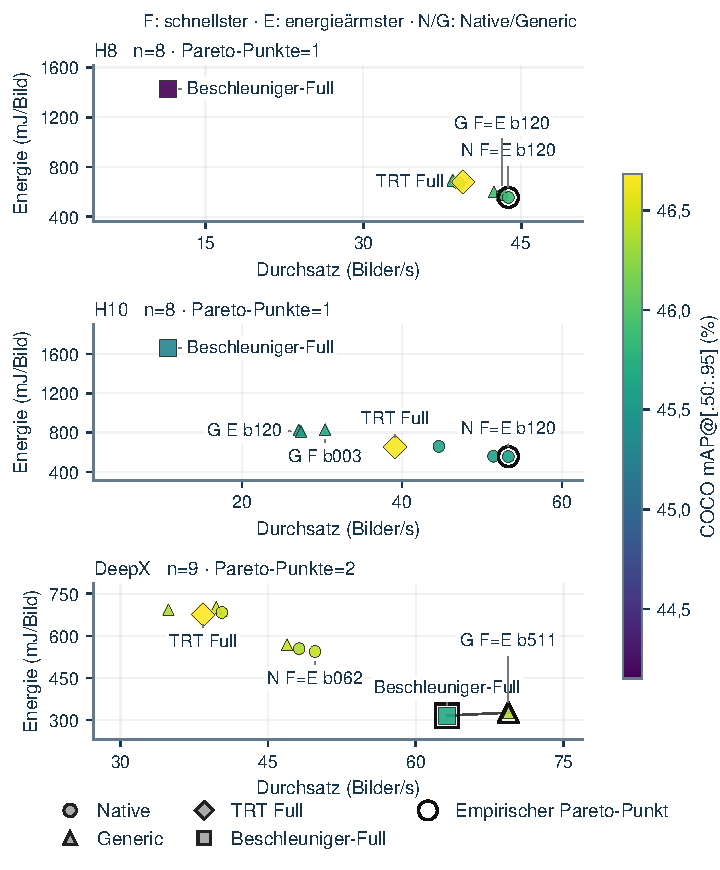
\includegraphics[width=4.8in]{9_resources/10_anhang/04_tradeoff_yolo11l.pdf}
\caption[YOLO11l-Konfigurationsraum]{YOLO11l: 25 gemessene Ausführungskonfigurationen, einschließlich Generic DeepX b511. H8 und H10 weisen jeweils einen ungefilterten Grenzpunkt auf, DeepX hingegen zwei. Die zusätzliche Split-Konfiguration übertrifft den schnellsten Full-Durchsatz um \num{9.9}\%, verbraucht dabei jedoch \num{3.5}\% mehr Energie pro Bild. DeepX Full bleibt die energieeffizientere Alternative.}
\label{fig:gallery:yolo11l}
\end{figure}
\clearpage
\begin{figure}[p]
\centering
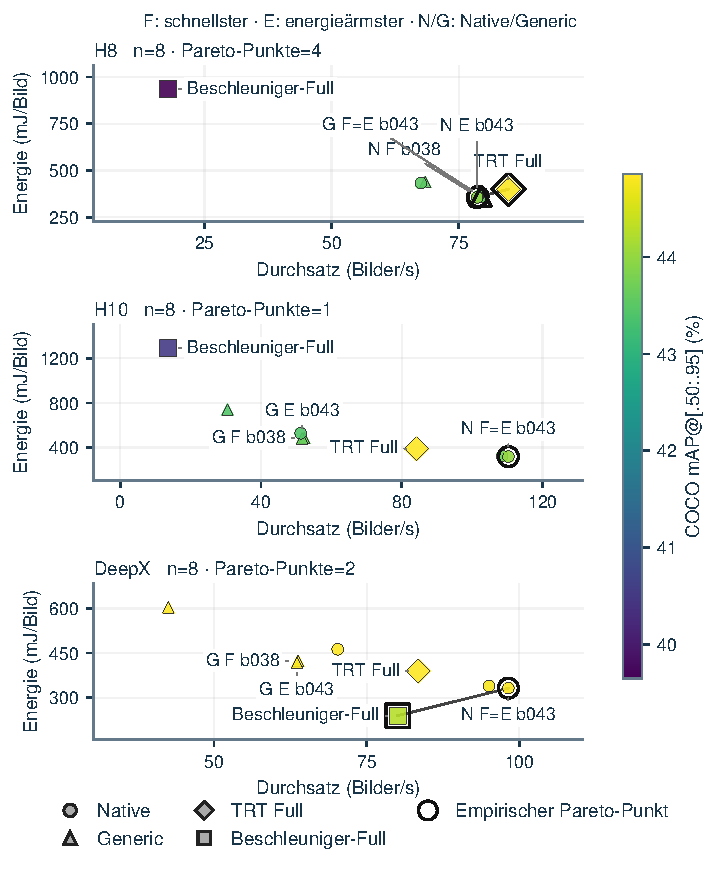
\includegraphics[width=4.8in]{9_resources/10_anhang/04_tradeoff_yolo26m.pdf}
\caption[YOLO26m-Konfigurationsraum]{YOLO26m: 24 gemessene Ausführungskonfigurationen. Auf H8 sind vier Konfigurationen nichtdominiert, auf DeepX zwei. Die über alle untersuchten Systeme schnellste Split-Variante auf H10 verbraucht weniger Energie als die schnellste Full-Konfiguration über alle untersuchten Systeme. DeepX Full verbraucht noch weniger Energie. Die Auswahl einer Full-Referenz nach Durchsatz minimiert deren Energieverbrauch nicht.}
\label{fig:gallery:yolo26m}
\end{figure}
\clearpage
\begin{figure}[p]
\centering
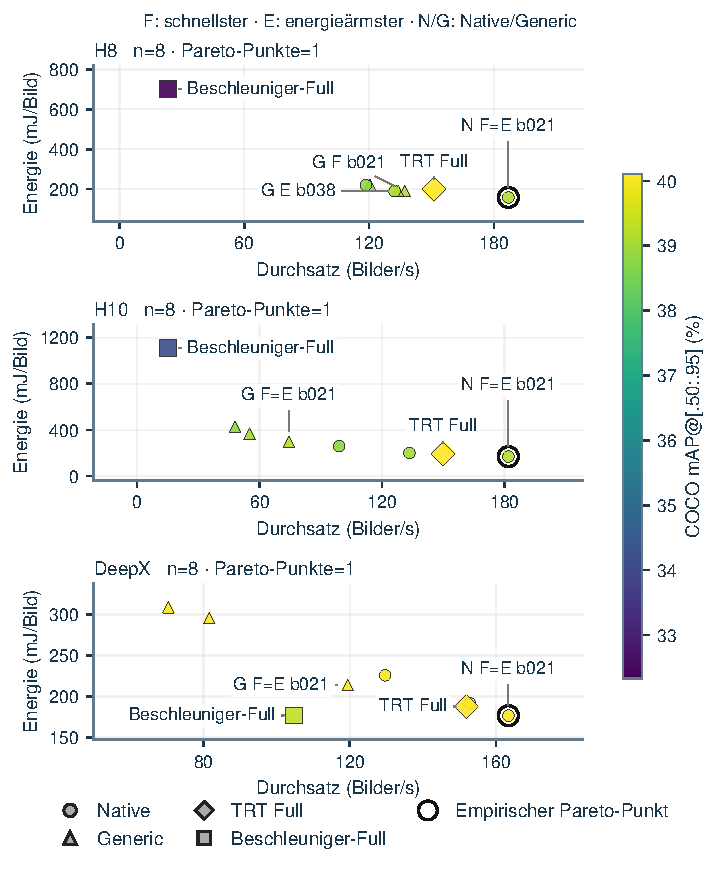
\includegraphics[width=4.8in]{9_resources/10_anhang/04_tradeoff_yolo26s.pdf}
\caption[Der Einsatzbereich von YOLO26s]{YOLO26s: 24 gemessene Ausführungskonfigurationen. Jeder Aufbau verfügt über genau eine Konfiguration auf der lokalen Zwei-Ziel-Grenze. Die schnellste Split-Konfiguration auf H8 verbessert sowohl den Durchsatz als auch den Energieverbrauch im Vergleich zur schnellsten Full-Konfiguration über alle untersuchten Systeme. Das Ergebnis ist auf die drei getesteten Schnitte pro Aufbau beschränkt und kann nicht jede gültige Graphgrenze charakterisieren.}
\label{fig:gallery:yolo26s}
\end{figure}
\clearpage
\begin{figure}[p]
\centering
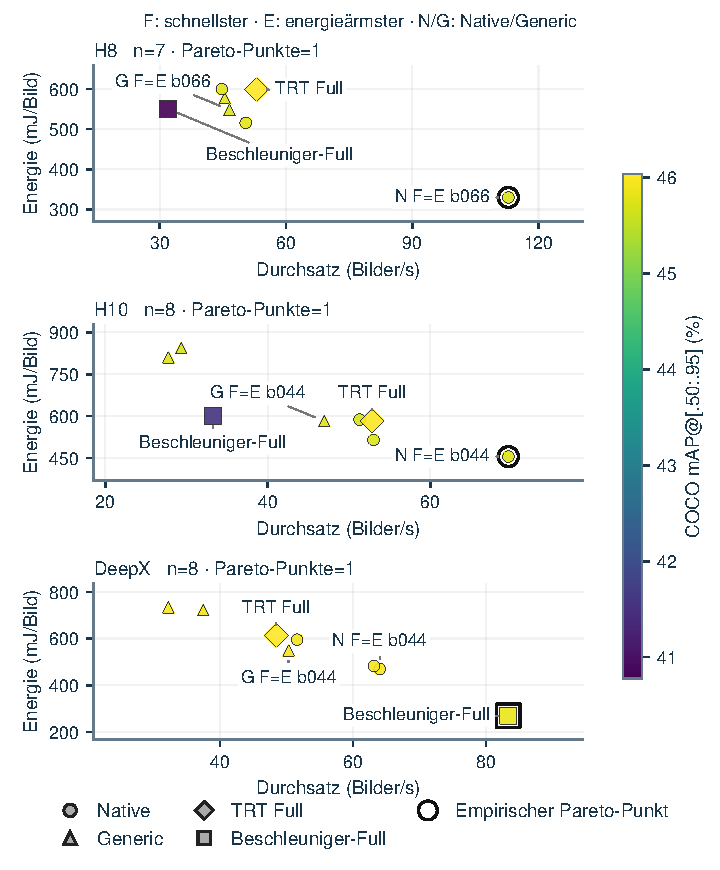
\includegraphics[width=4.79in]{9_resources/10_anhang/04_tradeoff_yolov7_paper.pdf}
\caption[YOLOv7-Konfigurationsraum]{YOLOv7: 23 grafisch dargestellte Ausführungskonfigurationen. Der Punkt Generic H8 b009 wurde weggelassen, da für ihn keine Energiebeobachtung vorliegt. Die schnellste Split-Konfiguration, H8 b066, übertrifft den Durchsatz der globalen DeepX Full-Konfiguration, verbraucht jedoch mehr Energie pro Bild. Die Grafik zeigt zudem die erheblichen Qualitätsunterschiede zwischen den Full-Pfaden des Beschleunigers. Frühere Studien zu Decodern und Vervollständigung tragen zur Erklärung verschiedener Aspekte des Ergebnisses bei und sind von diesen Beobachtungen getrennt zu betrachten.}
\label{fig:gallery:yolov7}
\end{figure}
\clearpage
